\chapter{Background}
\label{chap:background}
\section{Low-code development systems}
\label{sec:low-code}

In the previous chapter, we briefly described that our thesis aims to create a \emph{low-code data-driven} programming system.
In this section, we describe several existing systems that employ the low-code development approach to understand better how our resulting application fits into the low-code programming system landscape.
The low-code development approach can be defined as follows:
\begin{defn}[Low-code development approach]
	Defined by \citet{Pinho_Aguiar_Amaral_2023} as ``An approach for software development that uses tools that minimize (or eliminate) the number of lines of code written.''
\end{defn}
This definition accommodates a broad spectrum of tools and development systems.
The main category of these tools is \emph{visual programming tools} such as \emph{AppForge}~\cite{Yang_Gupta_Botev_Churchill_Levchenko_Shanmugasundaram_2008}, \citet{darklang} or \citet{mendix}.
The visual programming tools provide a Graphical User Interface (GUI), which allows users to create and modify software by interacting with the interface.
They differ in the style of UI, provided functionality, their intended use case, and other features, such as automatic deployment of the created software.

The next category of low-code development tools is \emph{Integrated development environments (IDEs)} with code generation capabilities.
For example, \citet{Rider} provides advanced context-aware code auto-completion alongside tools to generate boilerplate code and project scaffolding.
Code generation can also be provided by integrating \emph{Large Language Models (LLMs)} into existing IDEs, such as the~\citet{copilot} extension for the \citet{vscode} editor.

The last large category of low-code development tools is \emph{Static site generators (SSGs)}, which transform files written in a simple markup language into a static website.
A popular example of SSGs is the \citet{hugo} static site generator, which also provides tools for customizing the transformation process and supports custom templating.

To better understand the \emph{InterfaceSmith} system, we will describe four programming systems that greatly influence its design.
The \emph{Hypercard}, \emph{AppForge}, \emph{Darklang}, and \emph{Sketch-and-Sketch} belong to the category of visual programming tools.
Each system has a different intended use case, User Interface, and capabilities.
In Chapter~\ref{chap:design}, we explain \emph{how} these particular systems inspire the design of our system.

\subsection{Hypercard}
\emph{Hypercard} is a low-code development system created by Bill Atkinson for the Macintosh operating system. Apple released the program in 1987 at the
Macworld exposition in Boston~\cite{hyper_release}. Apple developed and maintained the program until 1998.
The popularity of the program ensured that similar programs and clones of Hypercard were created after its discontinuation.

The following summary of functionality is based on a manual for the Hypercard system written by~\citet{goodman_hypertext}.
The fundamental elements that the user creates are called \emph{cards}. Cards can hold data as text, have custom graphics, contain buttons, and implement custom behavior.
Users can implement the custom behavior using a scripting language called \emph{HyperTalk}. Then, users can group cards into \emph{stacks}. A~stack is a collection of cards with the same type of information.
The program saves a stack as a single file to the disk. Finally, users can distribute and modify these stacks.
Creation and modification of the card is done through the low-code interface. The program provides several options for the different card elements.
\begin{figure}[htbp]
	\centering
	\includegraphics[width=.8\linewidth]{img/hypercard−menu.pdf}
	\caption{Selection of a user level in the Hypercard preferences menu. (Image created using a Hypercard emulator~\cite{hypercard_emulator}.)}
	\label{fig:f}
\end{figure}

The program offers users a choice of a user level, as seen in figure \ref{fig:f}. The program changes the user interface's capabilities based on the selected user level.
The higher the selected user level, the more options the program enables and displays. A~selected level enables all previous-level options alongside other options and functionality.
Users can choose from five different user levels:
\begin{enumerate}
	\item \textbf{Browsing:} Enables no modification of cards and is mainly intended to be used to view the different cards inside a stack.
	\item \textbf{Typing:} Enables inserting and modifying text data inside the cards.
	\item \textbf{Painting:} Enables the creation of custom graphics inside the cards. The program provides different graphical options and tools.
	\item \textbf{Authoring:} Adds the ability to add buttons and fields. This way, the users can add card functionality without writing code.
	\item \textbf{Scripting:} Adds the ability to use the HyperTalk scripting language to modify the behavior of the different elements inside the cards.
\end{enumerate}
This allows the system to be adopted by a wide range of users, as less experienced users can learn to use the interface more easily and gradually increase their proficiency with the program without being overwhelmed by options.
Advanced users can set the highest user level and use the program in its entirety from the start.

\subsection{AppForge}
\emph{AppForge} is a low-code programming system presented by~\citet{Yang_Gupta_Botev_Churchill_Levchenko_Shanmugasundaram_2008}.
It is designed as a "what you see is what you get" (abbreviated as \emph{WYSIWYG}) platform for creating web applications using a low-code interface.
The system provides options for creating UI elements and automatically generates the necessary parts of a functional web application, such as the underlying database schemas and application logic \cite{Yang_Gupta_Botev_Churchill_Levchenko_Shanmugasundaram_2008}.

The users create UI elements using a low-code interface consisting of different menus, which we see in Figure~\ref{fig:appforge}.
The users manually create the two main types of elements, and they are \emph{Forms} and \emph{Views}.
Forms are used to add new data to the schema of a corresponding entity, and the Views are elements that display data from one or multiple database entities, and the user can modify how the data is displayed.
The system automatically creates a new database table for each new entity or when the user creates a View which displays data from multiple entities.

\begin{figure}[htbp]
	\begin{center}
		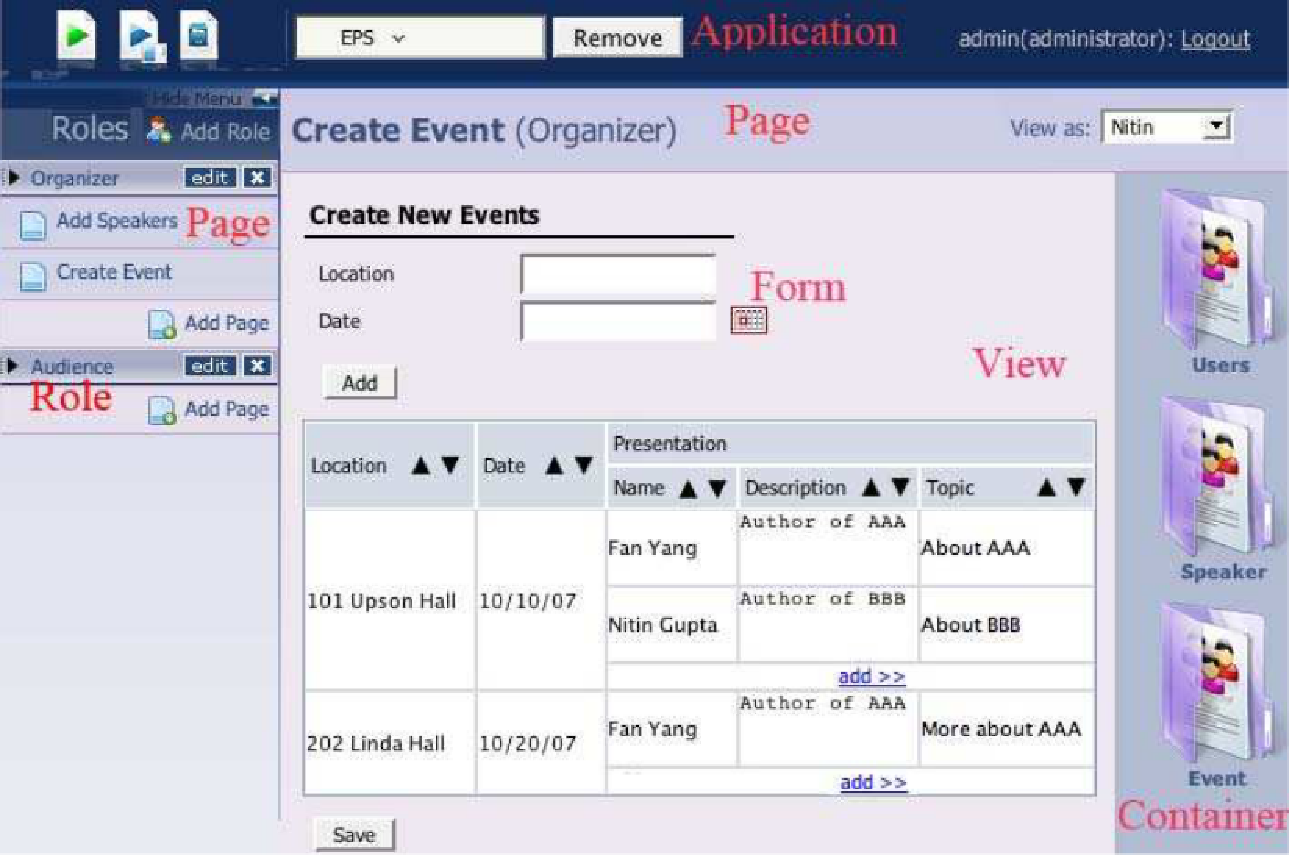
\includegraphics[width=0.95\textwidth]{img/appforge.pdf}
	\end{center}
	\caption{An example of AppForge's UI by \citet{Yang_Gupta_Botev_Churchill_Levchenko_Shanmugasundaram_2008} }
	\label{fig:appforge}
\end{figure}

%%TODO: add sources to descriptions to images

\subsection{Darklang}
\label{sec:darklang}
\citet{darklang} is a cloud-based low-code programming system for building web application backends created by Paul Biggar.
The original system's development was discontinued in 2023 and renamed Darklang-classic.

The following summary follows the official Darklang~documentation\footnote{\url{https://docs.darklang.com/} [visited on 2024-04-22][online]}.
The Darklang project consists of a low-code editor and a programming language. It also provides tools for creating persistent storage and for deployment.
The editor provides the service's main functionality. It consists of a canvas that displays the created application elements as draggable boxes as seen in Figure~\ref{fig:darklang}.
Each box provides options to modify the element. These options include different menus and input fields.
Some elements can be modified using the Darklang programming language to implement custom behavior.
The user can create program elements of the following categories:
\begin{itemize}
	\item HTTP handlers - definition of API endpoints
	\item Persistent storage - database creation and modification
	\item Workers - processing of background tasks
	\item Cron jobs - scheduled jobs with custom behavior
	\item REPL - a general-purpose programmable element
	\item Functions - a reusable element with custom behavior
\end{itemize}

\begin{figure}[htbp]
	\centering
	\includegraphics[width=1\linewidth]{img/darklang.pdf}
	\caption{Example of Darklang's drag-and-drop user interface. (Image created using the~Darklang-classic application~\cite{darklang}.)}
	\label{fig:darklang}
\end{figure}

By combining these elements, the users can create application backends of varying complexity.
The system automatically redeploys the entire application after the user creates and modifies a particular element.
This allows for an interactive style of development where changes made to the system are almost immediately visible.

\subsection{Sketch-and-Sketch - Output-directed programming}
\label{sec:odp}
\emph{Output-directed programming} is described by \citet{sketch-and-sketch} as
a programming paradigm where users construct plain text programs using mouse-based operations on the program's output.
The difference between this paradigm and other low-code programming approaches is that the source code is still the main representation of the program.
When making a change using the mouse-based operations is too hard or impossible, the user
can still change the output by directly changing the source code.
This approach is made possible thanks to the use of \emph{live synchronization} and \emph{trace-based program synthesis} as defined by \citet{output-directed-programming}

One example of a programming system that demonstrates this paradigm is called \emph{Sketch-and-Sketch} \cite{sketch-and-sketch,output-directed-programming}.
It is a browser-based application that provides a bimodal programming environment. It allows creating and modifying Scalable Vector Graphics (SVG) by directly manipulating the program's SVG output.
The application consists mainly of an editor window for the source code, a canvas window displaying the program's output, and a button to run the program.
After clicking on the canvas, the output is overlaid by context menus and \emph{widgets}, allowing users to modify the program's \emph{sub-expressions} and \emph{intermediate values} as seen in Figure~\ref{fig:sketch}.

\emph{Sub-expressions} refer to a certain syntactic scope of the program and the user can select and modify it~\cite{output-directed-programming}.
\emph{Intermediate values} are values produced at the intermediate execution steps of the program.
The program provides widgets for different types of intermediate values such as \emph{offset}, \emph{point}, or \emph{list} widgets.
Widgets can take the form of draggable boxes or input fields.

Another programming system implementing the direct manipulation paradigm is \emph{Transformic} introduced by \citet{Schreiber_Krahn_Ingalls_Hirschfeld_2017}.
It is a functional interpretation of the Morphic GUI Framework providing direct-manipulation functionality.

\begin{figure}[htbp]
	\centering
	\includegraphics[width=1\linewidth]{img/sketch.pdf}
	\caption{Example of Sketch-and-Sketch's user interface. (Image created using the~\citet{Sketch-n-Sketch-app}.) }
	\label{fig:sketch}
\end{figure}

\newpage
\section{Web Development}
In the previous section, we described the low-code development approach and several existing low-code development systems.
In this section, we introduce web development tools and technologies that we use for the \emph{InterfaceSmith} programming system or that influence its design and implementation.

To create a data-driven programming system, we must select a data representation format that is easy for users to obtain, understand, and modify.
We choose the \emph{JavaScript Object Notation format} for our input data representation, as it is widely used in web development, is easy to write and understand, and can be easily parsed.

Our programming system provides a GUI, and technologies such as the~\citet{elm} functional programming language influenced the nature of our implementation.
We do not use Elm directly, but we model our implementation after the~\citet{elm-arch} architecture, which is a simplified form of the programming model used by Elm.

To implement our programming system, we use the~\citet{fsharp} programming language alongside the~\citet{fable} compiler, which compiles the application into \emph{JavaScript},
which allows the application to run in a browser-based environment.

We use the \citet{feliz} library to implement the user interface of our programming system.
The \emph{Feliz} library provides a \emph{Domain-Specific Language (DSL)} for building \emph{React} user interface components and applications in F\#.
The \citet{react} library provides tools to create composable components, handle component-level storage and behavior, and handle the re-rendering of specific UI elements.

\subsection{The JavaScript Object Notation format}
The JavaScript Object Notation is defined by \citet{rfc8259} as a lightweight, text-based data interchange format.
It is language-independent and easy for both humans to read and write and machines to parse and generate.
JSON supports the following data types: \emph{Objects}, \emph{Arrays}, \emph{Numbers}, \emph{Strings}, \emph{Booleans}, and the \emph{null} type.
We can see an example of the JSON syntax in Figure~\ref{fig:json-example}

\begin{figure}[htbp]
	\caption {Example of the available JSON data types and the JSON syntax}
	\label{fig:json-example}
	\begin{lstlisting}
 { 
    "JsonObject" : {},
    "JsonList": [],
    "JsonString" : "Content",
    "JsonNumber": 0,
    "JsonBool" : true,
    "JsonNull": null
}
  \end{lstlisting}
\end{figure}

It is widely used in web development for transmitting data between the server and client-side web applications,
or used for configuration of different development tools.
Thanks to its popularity, many different parsers and other tools have been created to support its use, such as the \citet{simpleJson} library which we use in our implementation.

\subsection{Elm}
\citet{elm} is a functional programming language presented by \citet{Czaplicki_Chong_2013}.
It allows the creation of responsive graphical user interfaces by employing the
\emph{Functional Reactive Programming (FPR)} approach.
The functional reactive programming approach applies pure functional programming paradigms to time-varying values, as introduced by \citet{Elliott_Hudak_1997}.
Time-varying values can represent the input and output of the GUI or other information
channels, such as server requests. The applications to time-varying values are known
as \emph{signals}. Elm simplifies the approach of functional reactive programming,
by assuming that the signals are discrete. This means that it avoids unnecessary
recomputation when the signals are unchanged. Discrete change of a signal is called
an event. Events trigger the recomputation and the application is updated. Elm also
provides tools and abstractions to enable asynchronous computations.

The main categories of GUI elements in Elm are \emph{forms} and \emph{elements}.
\emph{Elements} represent a \emph{rectangular} GUI element with properties such as width and height. Elements
can contain data in a form of text, video or an image and can be composed together.
Forms on the other hand represent two dimensional elements of arbitrary shapes with
modifiable properties such as color and texture.

Reactive GUIs can be implemented by combining GUI elements and input signals.
Elm provides a range of primitive signals such as ”Mouse.clicks” which triggers on
mouse click. Some primitive signals may require arguments for their constructor such
as the ”Window.dimensions” signal.

\subsection{The Elm architecture}
\label{sub:elmish}

The \emph{Elm} architecture\citet{elm-arch}, or the \emph{Model View Update(MVU)} architecture, is a programming architecture for building web applications.
The architecture is inspired by Elm's FPR programming model but was simplified to make the programming model more usable and easier to learn, as stated by~\citet{news/farewell-to-frp_2024}.

\begin{figure}[htbp]
	\caption{Diagram of the Elmish Architecture}
	\label{fig:elm}
	\begin{tikzpicture}[
			node distance = 3cm,
			data/.style = {draw, rectangle, minimum width=2.5cm, minimum height=1cm},
			func/.style = {->, >=stealth, thick},
			every node/.style = {font=\small}
		]
		% Slightly increased node width and consistent naming
		\node[data] (model) {Model};
		\node[data, right=4cm of model] (ui) {User Interface};
		\node[data, below=3cm of ui] (msg) {Message};

		% More consistent arrow labels
		\draw[func] (model) -- node[above] {View: renders the UI} (ui);
		\draw[func] (ui) -- node[right] {UI event: creates a Message} (msg);
		\draw[func] (msg) -- node[below left, align=center]
		{Update:\\modifies Model based on the Message} (model);
	\end{tikzpicture}
\end{figure}

In Figure~\ref{fig:elm}, we can see a diagram representing the architecture.
The architecture consists of the following components:
\begin{itemize}
	\item \textbf{Model:} The \emph{Model} is a data-structure which keeps the state of the entire application. It
	      holds data and other necessary values that the application uses.
	      The data-structure is usually immutable.
	      This means that making changes to the state results in a creation
	      of an updated copy of the state which becomes the new state.

	\item \textbf{View:} View is a function which takes the current state of the application and creates a
	      graphical user interface. The interface usually consists of multiple GUI elements displaying the application state.

	\item \textbf{Update:} Update is a function which updates the model based on the inputs from the graphical user interface which calls the update function with a certain \emph{Message}.
	      Messages are similar to events in the Elm language. Each message represents a certain change to the model.
	      The update function updates the model based on the provided message and the current application state.
	      The message type is usually represented as a \emph{discriminated union}.
	      This enables the update function to use pattern-matching expressions to efficiently update the model.
\end{itemize}

\subsection{F\# and Fable}
\label{sub:Fable}

\citet{fsharp} is a functional-first programming language running on the .NET platform.
Although it is mainly a functional programming language, it allows the use of other paradigms, such as the imperative and object-oriented paradigms.
We chose F\# to implement our low-code programming system due to its strong type system, functional programming capabilities, and integration with the .NET ecosystem.
The reasons for this choice are further elaborated in Chapter~\ref{chap:implementation}.

\citet{fable} is a compiler capable of compiling programs written in F\# to multiple target languages.
One of the available target languages is JavaScript, and the compiler produces human-readable and formatted JavaScript code.
This enables the creation of web applications in a type-safe functional programming language while also enabling the use of tools and libraries from the wider JavaScript ecosystem.

The Fable compiler supports the use of some types from .NET Base Class and FSharp.Core libraries \cite{fable-comp} and attempts to compile these types to native JavaScript whenever possible.
This feature allows developers to leverage their existing knowledge of F\# and .NET while building web applications.

\subsection{React and Feliz}
The \citet{react} JavaScript library, initially developed by \emph{Facebook}, is used to create user interfaces for various target platforms, such as browsers or mobile devices.
The main idea behind this library is to simplify the development process by breaking down complex user interface elements into composable \emph{React components}.
Components are the main development units of React applications, and the library provides functionality to implement more complex per-component behavior, such as component-level storage or custom behavior of the UI elements.
Components can be implemented as \emph{class-based} or \emph{functional} using \emph{JSX}, which extends the standard JavaScript syntax.

The \citet{feliz} library provides a DSL to create functional React components in F\# Fable projects.
It combines the benefits of React, such as the ability to create composable UI elements, and the benefits of F\#, such as type safety and functional programming capabilities.
We can see an example of a component implemented in both JavaScript and React in Program~\ref{fig:react-feliz}.
\begin{listing}[htbp]
	\begin{center}
		\begin{lstlisting}
//Component implemented using JSX
function SimpleComponent() {
  return (
      <div>
          <p>JavaScript component</p>
      </div>
  );
} 

//Component implemented in F# using the Feliz DSL
[<ReactComponent>]
let SimpleComponent = 
  Html.div [
      Html.p "Feliz component"
  ]
  \end{lstlisting}
	\end{center}
	\caption{Comparison of JSX and Feliz syntax}
	\label{fig:react-feliz}
\end{listing}

